\documentclass[output=paper,modfonts,newtxmath,hidelinks,]{langscibook} 
\ChapterDOI{10.5281/zenodo.2545529}

\author{Kristina Mihajlović\affiliation{University of Arizona}\lastand{Małgorzata Ćavar\affiliation{Indiana University}}}

\title{Perception of Bosnian/Croatian/Serbian sibilants: Heritage U.S. vs. homeland speakers. A pilot study}

\abstract{Many dialectal varieties of Bosnian/Croatian/Serbian (BCS) show some level of merger of standard BCS alveolo-palatal and hard post-alveolar affricate series. This paper reports the results of a pilot study of the perception of BCS sibilants by heritage speakers in the United States. Twenty speakers were given a forced identification task. Results indicate that second generation heritage speakers are worse in performance than first generation heritage speakers. Additionally, heritage Croatian and Bosnian speakers across generations perform  worse than heritage Serbian speakers.

\sloppy
\keywords{heritage language, phonology, language change, merger, affricates, Bosnian/Serbian/Croatian}
}

\begin{document}
\maketitle 
\shorttitlerunninghead{Perception of BCS sibilants: Heritage U.S. vs. homeland speakers}
% \rohead{Perception of BCS sibilants: Heritage U.S. vs. homeland speakers}

 

\section{Introduction}

In \ili{Bosnian}/\ili{Croatian}/\ili{Serbian} (BCS), the standard varieties have a typologically relatively rare contrast between “hard” post-alveolar affricates (/tṣ, dẓ/, compare the transcription of \ili{Polish}  hard post-alveolars in \citet{Ladefoged-Disner2012}, or \ili{Slavic} transcription /tš, dž) and alveolo-palatal affricates (IPA transcription /tɕ, dʑ/).\footnote{The hard post-alveolars are notoriously ambiguous, not only because of the variation in their realization in BCS. If there is no merger, phonetically they are neither sensu stricto retroflexes (though compare phonological arguments in \citealt{Hamann2003}, e.g. for \ili{Polish}) nor typical palatoalveolars – although the sounds that have undergone merger are probably to be described as palatoalveoalars. We identify the non-merged, hard post-alveolars as /tṣ, dẓ/, symbols used in \citet[169]{Ladefoged-Disner2012} to describe \ili{Polish} hard post-alveolars, where the authors made a strong case for using a non-IPA symbol distinct from the available symbols.}$^,$\footnote{We will continue using the \ili{Slavic} symbols for the post-alveolar series for typographic reasons.} BCS has also hard-post-alveolar fricatives but no parallel alveolo-palatal fricatives. The inventory of sibilants in standard BCS is represented in \tabref{tab:mihajlovic:1}.


\begin{table}
\begin{tabularx}{\textwidth}{XCCC} 
\lsptoprule 
 Manner &   {     Dental} & { Post-alveolar} & {     Alveolo-palatal}\\
\midrule 
Fricatives & [s]~[z]& [ṣ]~[ẓ] \\
           & /s/~/z/& /š/~/ž/ \\
\tablevspace           
Affricates & [t͡s]   & [t͡ṣ]~[d͡ẓ] & [t͡ɕ]~[d͡ʑ]\\
           & /c/    & /č/~/dž/  & /ć/~/đ/\\
\lspbottomrule
\end{tabularx}
\caption{\label{tab:mihajlovic:1} Sibilants of standard varieties of Bosnian/Croatian/Serbian (phonetic symbols with Latin orthography between slashes)}
\end{table}


The contrast is cross-linguistically rare and, in fact, many dialectal varieties of BCS show different levels of merger of the two posterior places of articulation. The merging areas included Istria, northern Dalmatia, Dubrovnik, Boka Kotarska, the varieties spoken by the Muslims in Bosnia and Hercegovina, Catholics of eastern and northern Slavonia, areas of Banat and Timok-Lužnik, the dialect spoken in the capital of Croatia, Zagreb (\citealt{Stankiewicz1986}:107, and references therein, \citealt[296]{Ivic1958}, \citealt{Zygis2003} after \citealt{Ivic1958}). Included, because, given the changed geopolitical situation after the Yugoslav war, the expansion of \il{Stokavian@Štokavian} dialects at the cost of \il{Cakavian@Čakavian}Čakavian, and the increased prestige of \ili{Kajkavian} (spoken in the area of Zagreb), the situation described in before mentioned publications has evolved substantially. However, the authors of the current publication are not aware of any new comprehensive study of the current distribution of merging varieties. Other dialectal areas of BCS, such as Western Hercegovina, resist the merger entirely. Due to mobility of speakers between different dialectal areas, the current sociolinguistic situation is that of a daily interaction between speakers realizing the contrast in different ways and those not realizing the contrast. This is also the situation for the \isi{heritage language} as spoken in the U.S., which we investigate in this study. The influence of \ili{English} can potentially further facilitate the merger because one posterior place of articulation in \ili{English} (palatoalveolar /t͡ʃ, d͡ʒ/) corresponds to a two-way place of articulation contrast in BCS (alveolo-palatal /tɕ, dʑ/ and post-alveolar /tš, dž/). The current study contributes to our better understanding of the merger processes and \isi{language change} in general but also informs us of the strategies that native speakers adopt, first, when in close contact with different dialects and, second, with a dominant foreign language with conflicting phonological patterns.



\sectref{sec:mihajlovic:2} situates our study in the broader context of \isi{heritage language} research. 
In section \sectref{sec:mihajlovic:3}, the homeland situation is sketched. \sectref{sec:mihajlovic:4} is devoted to the methodology of the research and \sectref{sec:mihajlovic:5} provides the results. 
\sectref{sec:mihajlovic:6} relates the results back to the hypotheses and discusses the overall significance of the study while the paper is concluded in \sectref{sec:mihajlovic:7}.


\section{Heritage language studies context}\label{sec:mihajlovic:2}

The variety of BCS our study focuses on is the language of the \ili{Bosnian}, \ili{Croatian}, and \ili{Serbian} diaspora in the United States (in particular, Chicago and the surrounding areas, including Northern Indiana). Previous research on heritage languages suggests that the language of heritage communities differs in systematic ways from the language as spoken in the homeland communities. One factor here is the interaction between the L1 and L2 (in our case, the L2 is \ili{English}) sound systems (\citealt{Polinsky2018} and references therein). Additionally, in \isi{heritage language} communities, the close contact of different dialects must be considered. Due to several factors, such as heritage speakers’ geographical separation from homeland speech, there is less pressure from the standard language(s). This allows natural \isi{language change} to proceed unimpeded (or impeded to a much lesser degree) by prescriptive grammars, formal schooling and official media. Finally, it is often the case that heritage speakers do not reach the level of competence in their \isi{heritage language} that would be comparable with competence of homeland speakers \citep{Scontras-etal2015}. The language of the homeland is often not sufficient to serve as a universal communication tool in a different social context of the new country. Compensation strategies are developed to accommodate the needs of speakers, for example, code-switching. We believe that the situation of increased variation facilitates and accelerates \isi{language change}.



In \isi{heritage language} studies, there is no consensus concerning the definition of a \isi{heritage language} and heritage speaker. \citet{Polinsky2018} and \citet{Kelleher2010} provide overviews of several definitions of heritage speakers and \isi{heritage language}. \citet[1]{Scontras-etal2015} describe heritage speakers as “unbalanced bilinguals, simultaneous or sequential, who shifted early in childhood from one language (their \isi{heritage language}) to their dominant language (the language of their speech community).” The definition of a \isi{heritage language} can include a language that is acquired naturally at home, yet may be treated as a minority language outside of the home (\citealt{Polinsky2018}; see \citealt{Kupisch-etal2014} for further discussion of the definition of a heritage speaker). On the other hand, the term “heritage speaker” may also be used exclusively to describe bilinguals who were raised in a monolingual home (e.g., \citealt{Polinsky-Kagan2007}).



The current study will operate with the definition of a homeland speaker as an individual who natively speaks language A and still resides in their homeland country in which language A is widely spoken. On the other hand, we define a heritage speaker as someone who has lived in a new country in which their native language A is not widely spoken for a substantial amount of time, with the focus of their life interest moved to the new country;\footnote{For the purpose of our study, we adopted an arbitrary 7-year residence condition in the U.S. for the speakers of Generation 1 to exclude those new immigrants who would not have substantial exposure to \ili{English} and the \isi{heritage language} in the new country community.} if they do speak their \isi{heritage language}, it is usually reduced to being spoken in the home or with other speakers in a close-knit community. Heritage speakers are usually immigrants or displaced persons who have moved to a new country and their \isi{heritage language} skills often range widely, from fluent monolingualism or bilingualism to total language loss through attrition \citep{Scontras-etal2015}. This study includes speakers from each end of this spectrum as well as many who fall somewhere along the middle with respect to language attainment.



Another issue in heritage studies is the observed diachronic generation-to-generation change \citep{Otheguy-etal2007}. In our study, we have identified Generation 1 as speakers who acquired their \isi{heritage language} in the homeland natively, and Generation 2 as speakers who have primarily learned their \isi{heritage language} in the new country. We also included speakers who immigrated to the U.S. as very young children before the onset of formal education in the Generation 2 category.



Further, \citet{Polinsky2018} maintains that cross-linguistically, “immigrant and heritage varieties, separated from the ongoing change in the homeland, tend to retain features that are (or are perceived as) conservative” \citep[129]{Polinsky2018}. Whether or not the language changes within the same generation is also an area of interest. In our study we ask if the \isi{language change} is a function of time the speaker has spent within the new country. For example, in a large-scale analysis conducted using U.S. Census data of \ili{Spanish} speakers living in the United States, \citet{Veltman2000} found that “longer residence in the United States is associated with greater language shift.” \citep[66]{Veltman2000} In the context of our study, we will readdress these questions, the cross-generation differences and linguistic conservatism, in the discussion section.

% While 
Addressing the issue of conflicting phonological systems, \citet{Polinsky2018} assumes that heritage speakers generally use “the knowledge of contrasts from one language to the other only when such contrasts are useful,” and suppress such differences when unnecessary \citep[115]{Polinsky2018}. Using the concept of a distinction being “useful”, we are forced to adopt a perspective of a uni-directional influence of the dominant language influencing the \isi{heritage language}. In the context of the current study, this means that we would expect heritage BCS speakers with \ili{English} exposure to suppress their categorical distinction of alveolo-palatal vs. post-alveolar sibilants because \ili{English} lacks this place of articulation distinction and maintaining this contrast is not “useful” from the point of view of the acquisition of \ili{English}. One needs to observe that – although “usefulness” is primarily described in relation to the dominant language of the new country, in our case the “usefulness” of the contrast in the \isi{heritage language} itself can play a role, that is, in its \isi{functional load}. The contrast between post-alveolars and alveolo-palatals has a low \isi{functional load} in BCS.


\section{Sibilants of homeland speakers}\label{sec:mihajlovic:3}

BCS is a language continuum (called “macrolanguage” in Ethnologue) spoken in Croatia, Bosnia and Herzegovina, Serbia, and Montenegro with an estimated 15,260,000 speakers worldwide with considerable diaspora populations in the United States, Canada, and Australia (\citealt{Simons-Fennig2017}). \figref{fig:mihajlovic:1} shows the geographical area where the homeland BCS speakers are located in Eastern Europe.\footnote{\figref{fig:mihajlovic:1} is based on \url{https://upload.wikimedia.org/wikipedia/commons/3/31/Balkan_Peninsula.svg} by \url{https://commons.wikimedia.org/wiki/User:SilentResident} CC-BY-SA.}

\begin{figure}
% 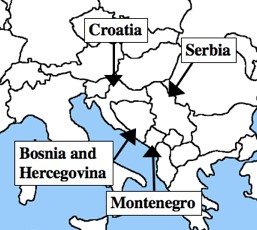
\includegraphics[height=.3\textheight]{figures/M_C_Figure 1.jpg}
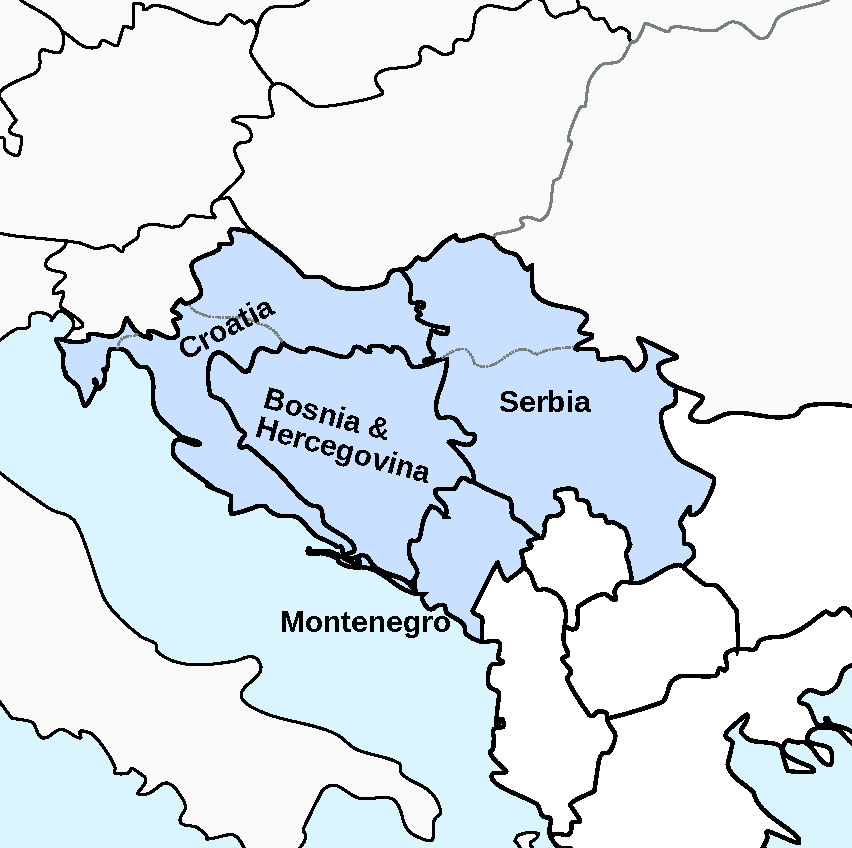
\includegraphics[height=.3\textheight]{figures/balkans.pdf}
\caption{\label{fig:mihajlovic:1}Southeastern Europe: Areas where homeland Bosnian/Croatian/Serbian is spoken}
\end{figure}

As shown in \tabref{tab:mihajlovic:1}, standard varieties of BCS contrast two posterior places of articulation for affricates. Conservative alveolo-palatals of BCS are articulated with an extreme raising of the tongue in the prepalatal area, while post-alveolars have the point of maximum constriction in the area of the alveolar ridge and just behind it, with the tongue body displaying no raising behind the constriction, see \figref{fig:mihajlovic:2}. This is different from \ili{English} where the palatoalveolars are articulated with a raised convex tongue but the raising is considerably less pronounced that in BCS alveolo-palatal sounds.

\begin{figure}
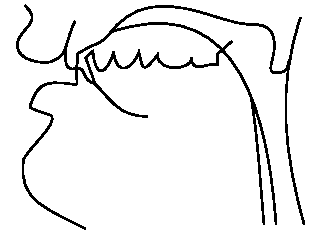
\includegraphics[width=.45\textwidth]{figures/MCFigure2left.pdf}
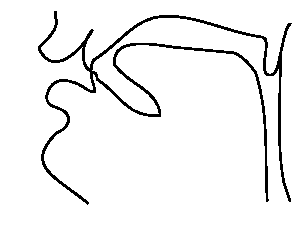
\includegraphics[width=.45\textwidth]{figures/MCFigure2right.pdf}
% 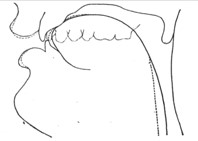
\includegraphics[width=.45\textwidth]{figures/MCFigure2left.jpg}
% 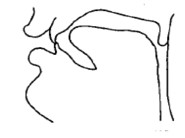
\includegraphics[width=.45\textwidth]{figures/MCFigure2right.jpg}
\caption{\label{fig:mihajlovic:2} Alveolo-palatals (left) and post-alveolars (right) in a non-merging variety (here: Serbian; adapted from \citealt{Miletic1958})}
\end{figure}


\citet{Skaric2009}, %when 
describing standard \ili{Croatian}, distinguishes between three pronunciation types. First, the classical, virtually non-existent pronunciation type preserves a clear contrast. Second, the received pronunciation, characterizes careful speech of educated speakers with remnants of the contrast, in particular, COG values partly overlapping for the two places of articulation.\footnote{COG (Center of Gravity) is in acoustics a measure for how high the frequencies in a spectrum are on average (at a particular point of time). COG provides a convenient dimension of comparison for sounds with a noise component. For example, denti-alveolar fricatives have their COG in higher frequencies and posterior fricatives.} Finally, the generally accepted pronunciation is that the places of articulation are completely merged. One has to bear in mind that the measures presented in \citet{Skaric2009} represent the speech of speakers recorded in Zagreb, thus in the merging dialectal area. The rendition of the standard may be heavily influenced by the local dialect and, thus, the picture might differ if the measurements were to include speakers in other \ili{Croatian} major cities. Whatever the details are, the point we want to stress is that some varieties of the homeland speech have merger or merger in progress, and that there is a lot of variation in the realization of the two posterior places of articulation for speakers of BCS in Europe.

\begin{figure}[b]
% 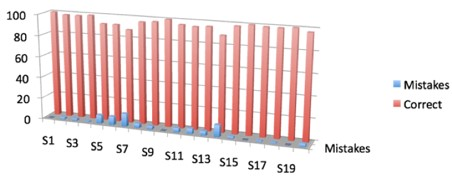
\includegraphics[height=.3\textheight]{figures/M_C_Figure 3.jpg}
\begin{tikzpicture}
            \begin{axis}[
                    ybar,
                    ylabel={\%},
                    xtick=data,
                    ylabel near ticks,
                    axis lines*=left,
                    ymin=0,
                    colormap/Greys,
                    cycle list/Greys,
                    xticklabels={pp1,pp2,pp3,pp4,pp5,pp6,pp7,pp8,pp9,pp10,pp11,pp12,pp13,pp14,pp15,pp16,pp17,pp18,pp19,pp20},
                    ticklabel style={font=\scriptsize\scshape},
                    bar width=.1cm,
                    xticklabel style={anchor=base,yshift=-1ex},
                    legend style={font=\footnotesize,at={(0.5,-0.2)},anchor=north},
                    legend columns=-1,
                    ylabel shift=-.15cm,
                    width=\textwidth,
                    height=5cm,
                    enlarge x limits={0.025},
                    nodes near coords,
                    nodes near coords style={text=black,font=\tiny},
                    ]
                \addplot+[
                     fill=Greys-F,draw=none
                    ] coordinates {(0,100) (1,98) (2,98) (3,99) (4,92) (5,92) (6,88) (7,96) (8,97) (9,100) (10,96) (11,95) (12,96) (13,89) (14,98) (15,100) (16,99) (17,99) (18,100) (19,97) };
                \addlegendentryexpanded{Accurate}              
                \addplot+[                                     
                     fill=Greys-M,draw=none
                    ] coordinates {(0,0) (1,2) (2,2) (3,1) (4,8) (5,8) (6,12) (7,4) (8,3) (9,0) (10,4) (11,5) (12,4) (13,11) (14,2) (15,0) (16,1) (17,1) (18,0) (19,3) };
                \addlegendentryexpanded{Mistakes} 
            \end{axis}                                                                           
\end{tikzpicture}
\caption{\label{fig:mihajlovic:3} Perception of alveolo-palatals versus hard post-alveolars in a forced-choice identification task (\citealt{Cavar-Hamann2008})}
\end{figure}

In our understanding of the “homeland” perception of the contrast between the two posterior places of articulation, we rely heavily on an earlier study by \citet{Cavar-Hamann2011}, who test{ed} speakers from Croatia and Bosnia and Hercegovina (to the exclusion of speakers from Serbia). The study was, however, guided by different research questions from those that we investigate today and used a different software and tokens recorded by a different speaker. In particular, \citet{Cavar-Hamann2011} was a study of inter-language perception and used tokens produced by a \ili{Polish} native-speaker. On the other hand, \ili{Polish} alveolo-palatal affricates are very similar, if not identical, to the \ili{Croatian} ones as articulated in non-merging dialects of Hercegovina. The tokens have also included alveolo-palatal fricatives, which are absent from \ili{Croatian}, to test if \ili{Croatian} speakers can use their ability to discriminate between alveolo-palatal affricates and hard post-alveolar affricates to perceive the contrast between \ili{Polish} alveolo-palatal fricatives and post-alveolar fricatives. Unlike for the \ili{German} control group, \ili{Croatian} participants perceived all contrasts – including those absent from BCS – at the level comparable with \ili{Polish} participants; see \figref{fig:mihajlovic:3}. Four subjects out of twenty reached 100\% accuracy in perception. The project also contained a production component.\footnote{This was a study conducted by \citet{Cavar-Hamann2008}.} The same \ili{Croatian} participants were recorded reading word lists containing \ili{Croatian} sibilants. The highest ratio of mistakes in perception (up to $12\%$) was observed in subjects who do not produce a stable contrast between soft and hard \isi{affricate} series in \ili{Croatian}. Both subjects with the relatively highest error level come from the same area (of Zadar). Interestingly, the relation is not reciprocal: not all participants who do not produce consistent contrast have a higher ratio of mistakes in perception.

The rendition of the posterior place contrast showed a lot of inter- and intra-speaker variation. One speaker was switching between a more standard pronunciation and the dialectal pronunciation from Pag, where standard alveolo-palatals are realized as palatal stops. Out of twenty participants, ten articulated a stable contrast, for five participants the contrast was not realized in a reliable fashion, and five others did not have the contrast. \tabref{tab:mihajlovic:2} shows the geographical origins of speakers.\footnote{Another useful consideration is how many of the speakers of either generation were speakers of a border variety of BCS – that is, a variety spoken near a political border. We did not collect this type of information and therefore cannot comment on this.}


\begin{table}
\begin{tabularx}{.9\textwidth}{rrSr}
\lsptoprule
{Štokavian} (coast) & {Štokavian} (Slavonia) & {Čakavian} & {Kajkavian}\\
\midrule
14 & 2 & 2 &  2\\
\lspbottomrule
\end{tabularx}
\caption{\label{tab:mihajlovic:2} Homeland Croatian speakers by dialectal area}
\il{Stokavian@Štokavian}
\il{Cakavian@Čakavian}
\il{Kajkavian} 
\end{table}


For those speakers whose pronunciation was not standard-like with two completely distinct categories, impressionistically five participants produced “hard” post-alveolars as more soft, four had alveolo-palatals shifted towards the “harder” series, three had variation in the production depending on whether the following vowel was front or back (only contexts of [e] and [a] were recorded). While only impressionistic descriptions are available at this point for all the original participants of the production study, it is clear that in homeland \ili{Croatian} the perception of the contrast is surprisingly good given the high ratio of speakers with either complete merger or inconsistent rendering.

The contrast between alveolo-palatal and another post-alveolar place of articulation is relatively rare cross-linguistically \citep{Maddieson1984}. The two sound series contrast, for example, in \ili{Chinese} languages, in \ili{Polish}, Serbo-\ili{Croatian} and Lower Sorbian, in \ili{Ubykh} and \ili{Abkhaz} (cf. \citealt{Ladefoged-Maddieson1996}). Some languages exhibit the contrast limited to individual manner of articulation and phonation type and/or enhance it with additional secondary articulations. From the functional point of view, it might be beneficial to merge the two series. Alve\-o\-lo-palatals involve higher level of raising from the neutral position than palato-alveolars (e.g. in \ili{English}), in contrast, “hard” post-alveolars require a much flatter tongue position than for the palato-alveolars, thus, a high degree of articulatory precision is necessary to maintain the contrast. Further, the two series are relatively similar auditorily. For example, in the interlanguage forced-choice identification task by \citet{Cavar-Hamann2011}, untrained \ili{German} native speakers achieved only $55\%$ accuracy.



Additionally, in BCS languages the contrast has a relatively low \isi{functional load}. To our knowledge, there are no studies focusing on the \isi{functional load} of the contrast, but homeland(s) grammars (such as e.g. \citealt{Brozovic1991}) cite usually only a couple of relevant minimal pairs.\footnote{E.g. \textit{spavaćica} `pajamas' vs. \textit{spavačica} `woman, sleeping'. Other minimal pairs include \textit{posećen} `visited' vs. \textit{posečen} `cut', \textit{veće} `bigger' vs. \textit{veče} `evening' (\ili{Serbian}), \textit{kuće} `houses' vs. \textit{kuče} `puppy' (\ili{Bosnian}), and \textit{ćar} `benefit', `gain' (\ili{Bosnian}) vs. \textit{čar} `charm'; data retrieved from \url{https://forum.unilang.org/viewtopic.php?t=3028}.} The frequency of letters in \ili{Croatian} generated by a character counter lists the letters \textit{đ, ć, č, (d)ž} among the least frequent in \ili{Croatian} – not counting the foreign letters \textit{y, w, x}, and \textit{f} – with the following percentages in \ili{Croatian}: \textit{đ} at $0.20\%$, \textit{ć} at $0.49\%$, \textit{č} at $0.92\%$, \textit{ž} at $0.47\%$, all this bearing in mind that \textit{ć} occurs in some frequent function words like \textit{hoću} `will.\textsc{1sg}’.\footnote{We used the following character counter: \url{https://www.sttmedia.com/characterfrequency-croatian}.} While the frequency of the letters in a written corpus cannot be interpreted directly to evaluate the frequency of sounds (for example, because \textit{ž} is used in the representation of both the fricative ([ž]) and \isi{affricate} ([dž]), it indicates that the sounds represented by the letters are at the bottom rank with regards to their \isi{functional load}. No striking differences are expected between \ili{Croatian} and other standard varieties. It is our understanding that low \isi{functional load} might potentially facilitate the merger (cf. \citealt{Wedel-etal2013}).


\section{Methodology}\label{sec:mihajlovic:4}

The study was guided by a number of research questions. First, we are interested, given the intra-language structural pressure and the influence from the contact language, whether or not Generation 2 merges more than Generation 1.


\begin{exe}
\exi{H1:}  Second-generation speakers merge more than first-generation   speakers.
\end{exe}


Further, we are also interested in the influence of the dominant \ili{English} on the speech of Generation 1 heritage speakers, in particular we have assumed that for Generation 1 there will be a correlation between the length of the stay in the U.S. and the amount of merger:


\begin{exe}
\exi{H2:}  First-generation speakers are more likely to perceptually merge   the two categories the longer they have spent in the United   States.
\end{exe}


Finally, we want to verify earlier findings from a pilot study of \citet{Cavar-etal2016} that hard post-alveolars tend to be realized as (more) soft while alveolo-palatals are relatively stable in the merger; see \REF{ex:mihajlovic:1a}. The other possible scenario in this merger process would be that both categories move towards the halfway point between alveolo-palatals and original post-alveolars (e.g. in terms of COG) to produce a palato-alveolar sound, as in \REF{ex:mihajlovic:1b}.

\ea\textbf{Merger scenarios}
   \ea\label{ex:mihajlovic:1a}
alveolo-palatals      → alveolo-palatal\\
        hard post-alveolars → alveolo-palatal
\ex\label{ex:mihajlovic:1b}  alveolo-palatals       → palatoalveolars\\
        Hard post-alveolars → palatoalveolars
\z
\z

\begin{exe}
\exi{H3:}  In the merging contrast, alveolo-palatals are more salient perceptually and are perceived with greater accuracy than post-alveolars.
\end{exe}

The study included a production part (a reading task) and a perceptual experiment. This paper reports the preliminary results of the perceptual study.

In the perception study, participants were asked to listen to syllables containing one \isi{sibilant} in various vowel contexts, either VC, CV, or VCV. Participants were asked to listen to syllables containing one of six \isi{sibilant} sounds and then forced to identify which sound of a pair they perceived it to be. By utilizing a forced representation task in the experiment, participants were required to make a decision on their perception of the sound regardless of how confident they feel on their decision. During the experiment, the reaction time was also recorded, but so-far not analyzed.



The tokens were recorded by a female native speaker from Hercegovina who produces a stable contrast between alveolo-palatal and post-alveolar places of articulation in her speech. The native speaker read a list of nonce words composed of a \isi{sibilant} sound surrounded by the same vowel on either side (e.g. /eće/, /eče/, /eše/, etc.). The data were obtained through a forced-choice identification task made with Paradigm (experiment adapted from \citealt{Lee-Jongman2016}) and ran on a Lenovo laptop with headphones on. \tabref{tab:mihajlovic:3} details the methods used to derive the 36 stimuli for the experiment; 6 stimuli came from each of the 6 sounds in the first column. Each stimulus was repeated once for a total of 72 tokens.\footnote{/c/ and /š/ were included in the perception experiment to act as a control set to contrast with the merging series. As such, the stimuli used for /c/ came from a different native speakers' recording and the sound was extracted independently with no surrounding vowel information. The stimuli for /š/ came from the original native speaker, but less environments were included. As expected, the perception of both sounds was perfect for all speakers across all dialects and all generations (see \tabref{tab:mihajlovic:7}) because neither /c/ nor /š/ are merging in any variety of BCS we are aware of.} The final column gives the spliced stimuli which were used in the perception experiment.

\begin{table}
\begin{tabularx}{\textwidth}{llXQQ}
\lsptoprule
 \textbf{Sound} &  \textbf{Token environment} &  \textbf{Tokens} &  \textbf{Stimulus environment} &  \textbf{Spliced stimuli}\\
\midrule
{ć} & \#\_VC & {ćes}\newline ćas & \#\_V & {će}\newline ća\\
& CV\_\# & {seć} \newline sać & V\_\# & {eć} \newline  ać\\

\tablevspace 
& CV\_V\# & {seće}\newline saća & V\_V & {eće}\newline aća\\

\tablevspace
č & CV, VC, VCV & identical as ć & identical as ć & če, ča, eč, ač, eče, ača\\
{đ} & CV, VC, VCV & identical as ć & identical as ć & đe, đa, eđ, ađ, eđe, ađa\\
dž & CV, VC, VCV & identical as ć & identical as ć & dže, dža, edž, adž, edže, adža\\
c & C &  &  & c\\
{š} & \#\_VC & {šes} \newline šas & V\_\# & še, ša\\
& CV\_V\# & seše & V\_V & eše\\
\lspbottomrule
\end{tabularx}
\caption{\label{tab:mihajlovic:3} Stimuli used in the perception experiment}
\end{table}


Tokens were presented using headphones connected to a computer. Participants were tasked with indicating what they hear by clicking either the left arrow for /ć/, /đ/ or /c/, or the right arrow for /č/, /dž/ or /š/, as shown in \figref{fig:mihajlovic:4}.

\begin{figure}[t]
% 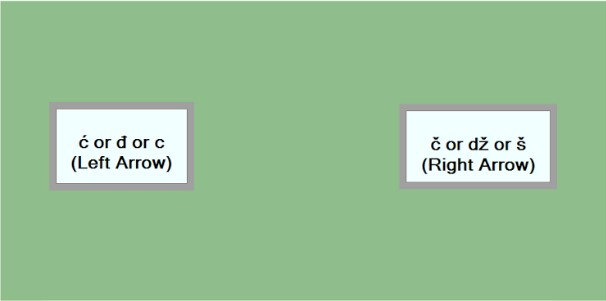
\includegraphics[height=.3\textheight]{figures/M_C_Figure 4.jpg}
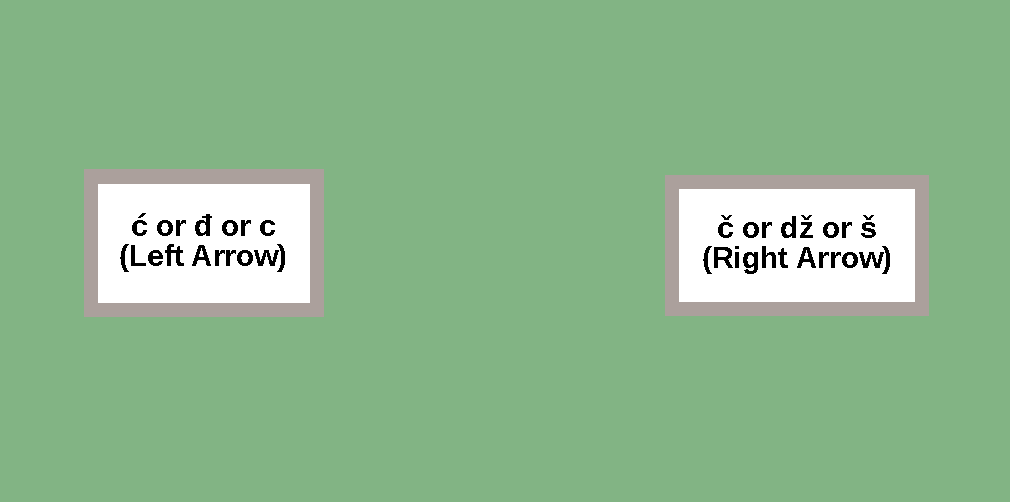
\includegraphics[height=.3\textheight]{figures/MCFigure4.pdf}
\caption{\label{fig:mihajlovic:4} Perception experiment design}
\end{figure}

The symbols correspond to standard orthographic form in the Latinica (\ili{Latin}-based) alphabet. While the post-alveolar sounds in the merging series (/č, dž/) were grouped together and the alveolo-palatal sounds (/ć, đ/) were grouped together, there was no other correspondence between the direction of the arrow and any phonetic characteristic of the sound, especially in the arbitrary case of /c/ and /š/. Participants were asked to complete a brief demographic questionnaire in which they provided information, for example, on the language background of their parents. The language background survey asked participants to disclose their

\begin{enumerate}
\item sex, 
\item age, 
\item first languages (“ones you’ve spoken since you can remember”), 
\item birth city, state, and country,
\item childhood home (“Where did you spend your childhood, if different than the above?”), 
\item year of arrival to United States (“If you moved to the U.S., when did you come and to what city and state?”), 
\item parents’ home (“Where did your parents/guardians spend their childhood (city, state, and country)?”),
\item other homes (“other cities which you have visited/lived for more than three consecutive months”), including location (city, state, country), duration, and age.
\end{enumerate}

Then for each language/dialect known (including native), participants were asked to provide 

\begin{enumerate}
\item[9.] age of acquisition, 
\item[10.] years of experience with this language, and 
\item[11.] usage questions such as:          
  “What percent of the time do you use this language?”,    
  “Who do you typically speak this language with? (please list your     relationship with people, but no names)”, “Where are these people usually from?”,
  “In what environment(s) do you usually use this language? (Or when do     you usually get a chance to speak this language?)”,
  “How important do you think it is for you to speak this language?", 
  “Please indicate your abilities in each of the four areas in this language:” Areas: Speaking, Listening, Reading, Writing; Abilities: Poor, Fair, Good, or (Near)-Native?
\end{enumerate}

A complete copy of the questionnaire is available upon request from the first author.

We defined first generation (Gen1) speakers ($N=11$) as those who moved to the United States at seven years of age or older because children start their formal education in the homeland at the age of 7 and from that time on they become increasingly exposed to normative language education. Generation 2, in contrast, includes speakers who emigrated as very young children (before formal schooling began), as well as those who learned their \isi{heritage language} in the current country of residence from their Generation 1 parents. In our study, we have investigated only Generation 1 and Generation 2 speakers.



20 speakers participated in the study, most of them ($N=18$) women. The age of participants ranged from 20 to 78 and was correlated with their generation (Generation 1 versus Generation 2), where Generation 1 was older and Generation 2 was younger. Generation 1 was comprised of 11 participants while Generation 2 was comprised of 9 participants. We divided the participant group into Bosnians, Croatians, and Serbians, based on the place of birth, or the place of birth of the parents (for Generation 2). Half of all participants ($N=10$) were included in the \ili{Serbian} group, six in the \ili{Bosnian} and {Herzegovinian} group, and four in the \ili{Croatian} group. \tabref{tab:mihajlovic:4} provides a summary of speaker breakdown.\footnote{Gen 1 age mean: $45.73$ (SD $18.91$); Gen 2 age mean: $25.00$ (SD 11.36).}


\begin{table}
\begin{tabularx}{\textwidth}{XXl}
\lsptoprule
&  \textbf{Generation 1} &  \textbf{Generation 2}\\
\midrule
female/male count & F = 10, M = 1 & F = 8, M = 1\\
age range & 20--57 & 20--78\\
dialect breakdown & 2 B, 3 C, 6 S & 4 B, 1 C, 4 S\\
\lspbottomrule
\end{tabularx}
\caption{\label{tab:mihajlovic:4} Participants overview; B = Bosnian, C = Croatian, S = Serbian}
\end{table}

\section{Results}\label{sec:mihajlovic:5}

The following sections present the findings. \sectref{sec:mihajlovic:5.1} presents the basic descriptive statistics, \sectref{sec:mihajlovic:5.2} compares the results for Generation 1 and Generation 2 speakers. In \sectref{sec:mihajlovic:5.3}, the results of the current study are compared with the available results of homeland speakers in \citet{Cavar-Hamann2011}. \sectref{sec:mihajlovic:5.3} addresses the length of stay in the U.S. as a potential factor influencing the merger in the first generation of immigrants and \sectref{sec:mihajlovic:5.4} looks at the potential differences in the perception of different categories.


\subsection{General results}\label{sec:mihajlovic:5.1}

Let us start with the ratios of incorrect responses for the three sub-groups of participants depending on the area of origin across the two generations. The data is further divided with respect to the type of sound – non-merging hard post-alveolars (/š/), merging hard post-alveolars (/tš, dž/), and merging alveolo-palatals (/ć, đ/).


\begin{table}
\begin{tabularx}{\textwidth}{lQr@{.}lr@{.}l}
\lsptoprule

\textbf{Area of origin} &  \textbf{Sound group} &  \multicolumn{2}{l}{\textbf{Gen1}} &  \multicolumn{2}{l}{\textbf{Gen2}}\\
\midrule
{ Serbia} & Non-merging hard post-alveolars & $2$&$8\%$ & $0$&$0\%$\\
& Merging hard post-alveolars & $4$&$2\%$ & $41$&$7\%$\\
 & Merging alveolo-palatals & $6$&$9\%$ & $33$&$3\%$\\
 \midrule
 & All & $4$&$6\%$ & $25$&$0\%$\\

\tablevspace 
 \midrule
{ Bosnia} & Non-merging hard post-alveolars & $0$&$0\%$ & $4$&$2\%$\\
& Merging hard post-alveolars & $4$&$2\%$ & $52$&$0\%$\\
 & Merging alveolo-palatals & $4$&$2\%$ & $47$&$9\%$\\
\midrule
 & All & $2$&$8\%$ & $34$&$0\%$\\

\tablevspace
 \midrule
{ Croatia} & Non-merging hard post-alveolars & $2$&$8\%$ & $0$&$0\%$\\
& Merging hard post-alveolars & $30$&$6\%$ & $8$&$3\%$\\
 & Merging alveolo-palatals & $36$&$1\%$ & $83$&$0\%$\\
\midrule
 & All & $23$&$1\%$ & $30$&$6\%$\\ 
%  \tablevspace
%  \midrule
% { Heritage speakers} &  &  \multicolumn{2}{l}{} & $360$&$0\%$\\
\lspbottomrule
\end{tabularx}
\caption{\label{tab:mihajlovic:5} Percent of incorrect answers by area of origin, generation and sound type}
\end{table}


Due to the complex geolinguistic situation in the countries of former Yugoslavia, it was sometimes impossible to unambiguously identify the exact dialect spoken by participants in Generation 1, instead we use the area of origin as the variable. Generalized Linear Mixed Model (GLMM) analysis was conducted and the area of origin did not turn out to be a significant predictor in our data with $p=0.24$ (model also includes generation, sound type, sound environment, age, and number of years since the acquisition of \ili{English}). \ili{Croatian}-origin participants’ responses are marginally different from the \ili{Serbian} group ($p=0.099$). However, when looking at raw percentages, certain tendencies in the data can be observed. In particular, in the first generation \ili{Croatian}-origin participants merge more than other groups. This difference is levelled in second generation.


\subsection{Do the second-generation speakers merge more than the first-generation speakers?}\label{sec:mihajlovic:5.2}

The absolute number of incorrect responses is much higher in Gen2 than in Gen1 in total as well as for each subgroup of participants separately. A GLMM analysis has been conducted controlling for generation as a factor. The difference between Gen1 and Gen2 is statistically significant ($p=0.005$). For \ili{Serbian}-origin participants, the difference between Gen1 and Gen2 is significant with $p=0.046$, highly significant for \ili{Bosnian} speakers ($p=0.001$), however, this difference turned out to be insignificant for \ili{Croatian}-origin participants ($p=0.739$).


\subsection{Does the duration of the stay in the United States influence the level of merger in Gen1 speakers?}\label{sec:mihajlovic:5.3}

With regards to H2, in which we predicted that the longer the duration of stay in the United States, the more likely a speaker is to merge the categories. We found that our results do not support this hypothesis. In fact, the duration of stay in the U.S. in Generation 1 speakers had no effect on the level of merger ($p=1$). \figref{fig:mihajlovic:5}, which was added in response to a reviewer’s request, shows this lack of correlation between length of stay in the United States and accuracy of merging tokens. For our purposes, a higher level of merger is indicated by a lower accuracy of properly identifying merging tokens.

\begin{figure}
% 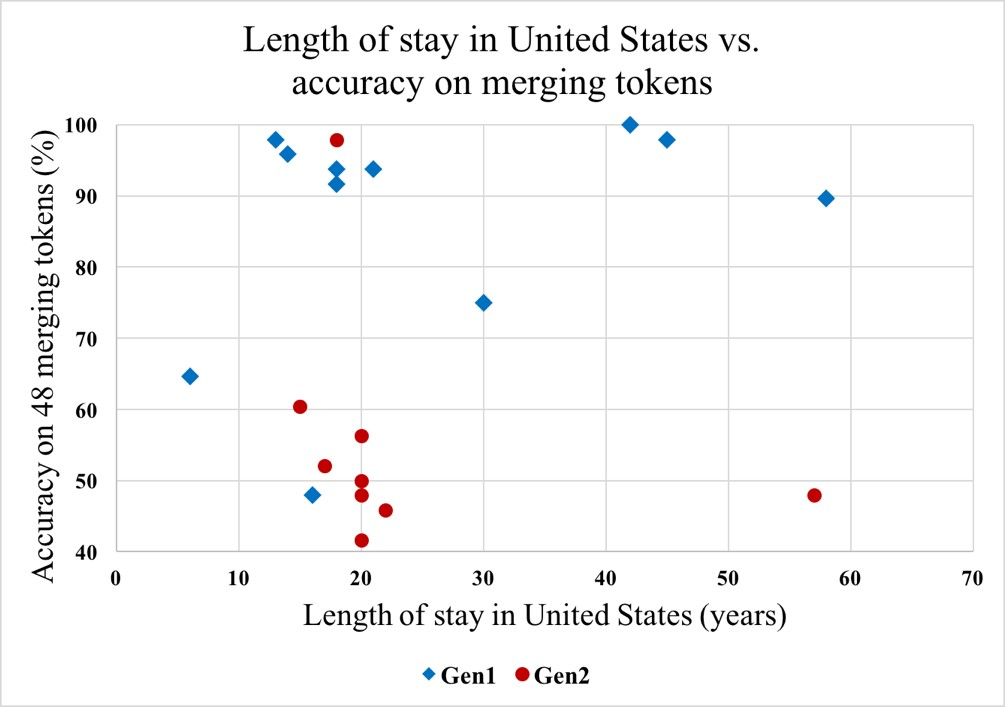
\includegraphics[height=.3\textheight]{figures/M_C_Figure 5.jpg}
\caption{\label{fig:mihajlovic:5} Length of stay in the U.S. vs. accuracy on merging tokens}
\begin{tikzpicture}
    \begin{axis}[
        scatter/classes = {
            GEN1={mark=diamond*,lsMidBlue},
            GEN2={mark=*,lsRed}
        },
        ylabel={Accuracy on 48 merging tokens (\%)},
        xlabel={Length of stay in the U.S. (years)},
        ymin=0,
        ymax=100,
        legend columns=1,
        legend style={legend pos=outer north east,cells={anchor=east}},
        legend entries={Generation 1,Generation 2}
    ]
    \addplot[scatter, only marks, scatter src=explicit symbolic] coordinates {
    (6,64.5833333333333)   [GEN1]
    (16,47.9166666666667)  [GEN1]
    (45,97.9166666666667)  [GEN1]
    (13,97.9166666666667)  [GEN1]
    (18,93.75)             [GEN1]
    (21,93.75)             [GEN1]
    (30,75)                [GEN1]
    (42,100)               [GEN1]
    (58,89.5833333333333)  [GEN1]
    (14,95.8333333333333)  [GEN1]
    (18,91.6666666666667)  [GEN1]
    (20,41.6666666666667)  [GEN2]
    (20,47.9166666666667)  [GEN2]
    (15,60.4166666666667)  [GEN2]
    (20,56.25)             [GEN2]
    (18,97.9166666666667)  [GEN2]
    (17,52.0833333333333)  [GEN2]
    (22,45.8333333333333)  [GEN2]
    (57,47.9166666666667)  [GEN2]
    (20,50)                [GEN2]
    };    
% %     \addlegendentries 
    \end{axis}
\end{tikzpicture}
\end{figure}

\subsection{Is either of the merging categories more “difficult"?}\label{sec:mihajlovic:5.4}

Further, we have looked at the identification ratios across sound categories. Post-alveolars are split into the affricates (potentially merging with alveolo-palatal series) and fricatives (which do not have corresponding alveolo-palatal fricatives, thus, do not merge with any other existing category). While the identification of [š] (a non-merging category) is, as expected, close to $100\%$, for all heritage speakers -- Generation 1 and 2 -- the correct identification of voiceless \isi{affricate} categories is only slightly above $80\%$.



\figref{fig:mihajlovic:6} shows the perception accuracy by sound type for voiceless sounds. In \figref{fig:mihajlovic:7}, the sound type accuracy for each of the three sound types, alveolo-palatal merging, post-alveolar non-merging, and post-alveolar merging, is represented for the two generations separately. The dashed line represents the perception accuracy of Generation 1, while the solid line represents the accuracy of Generation 2. The accuracy of the post-alveolar [š] is near 100\%, which was expected as this sound is non-merging.

\begin{figure}
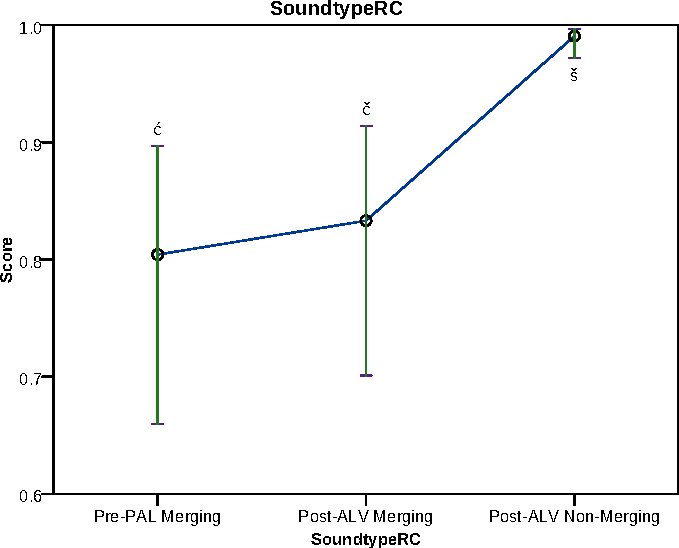
\includegraphics[height=.3\textheight]{figures/MCfig6.pdf}
\caption{\label{fig:mihajlovic:6} Perception in heritage speakers: alveolo-palatal (in the above graph, represented by ‘pre-palatal’ merging = [ć], post-alveolar non-merging = [š], post-alveolar merging = [č] (all heritage participants)}
\end{figure}

\begin{figure}
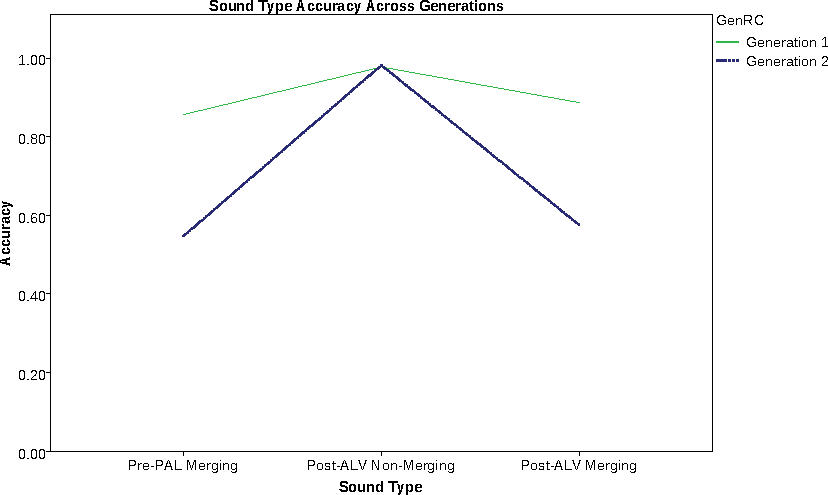
\includegraphics[height=.3\textheight]{figures/MCfig7.pdf}
\caption{\label{fig:mihajlovic:7} Accuracy of sound types. Key: dashed = Gen 1, solid = Gen 2; Alveolo-palatal (in the above graph, represented by ‘pre-palatal’) merging = [ć/đ], post-alveolar non-merging = [š], post-alveolar merging = [č/dž]}
\end{figure}

Contrary to what was expected, post-alveolar affricates and alveolo-palatal affricates reached similar level of accuracy in the identification task, however, the difference in the identification of the two merging categories was not significant, neither for Generation 1 nor Generation 2. /š/ is correctly identified more often than both alveolo-palatal /ć/ and post-alveolar /č/, for both generations and the difference is statistically relevant, see \tabref{tab:mihajlovic:7}.

\begin{table}
% \begin{tabularx}{\textwidth}{Qlr@{.}lr@{.}l}
% \lsptoprule
% &  &  \multicolumn{2}{l}{\textbf{Gen1} ($p$)} &  \multicolumn{2}{l}{\textbf{Gen2} ($p$)}\\
% \midrule
% alveolo-palatal merging \& post-alveolar merging & ć vs. č & $0$&$386$ & $0$&$671$\\
% \tablevspace
% alveolo-palatal merging \& post-alveolar non merging & ć vs. š & $0$&$001$* & $0$&$000$\\
% \tablevspace
% post-alveolar non-merging \& post-alveolar merging & š vs. č & $0$&$004$* & $0$&$000$*\\
% \lspbottomrule
% \end{tabularx}
\begin{tabularx}{\textwidth}{p{4.5cm}lXX}
\lsptoprule
&  &  \textbf{Gen1} (OR[CI]) &  \textbf{Gen2} (OR[CI])\\
\midrule
alveolo-palatal merging\newline\& post-alveolar merging & ć vs. č & {}-\newline $p=0.386$ & {}-\newline $p=0.671$\vspace{20pt}\\
alveolo-palatal merging\newline\& post-alveolar non merging & ć vs. š & $10.96$\newline[$2.85$--$42.06$]\newline $p=0.001$*& $42.69$\newline[$9.89$--$184.38$]\newline $p=0.000$*\vspace{6pt}\\
post-alveolar non-merging\newline\& post-alveolar merging & š vs. č & $7.49$\newline[$1.07$--$29.05$]\newline $p=0.004$* & $48.18$ \newline [$11.17$--$207.89$]\newline $p=0.000$*\\
\lspbottomrule
\end{tabularx}
\caption{\label{tab:mihajlovic:7} Statistically relevant difference in the perception between sound type for voiceless sounds (OR = odds ratio, CI = confidence interval)}
\end{table}



The goodness of the perception of alveolo-palatals is not statistically better or worse than the perception of post-alveolar affricates. This finding does not support the hypothesis that alveolo-palatals are more stable than post-alveolar merging affricates, which was based on the pilot data from an articulatory study by \citet{Cavar-etal2016}. Non-merging categories (posterior fricatives) are sticking away from the rest in terms of accuracy of identification. Non-merging post-alveolars are approx. 7.49 times more likely to be identified correctly than merging post-alveolars and approx. 10.96 times more likely to be identified correctly than alveolopalatals.



\section{Discussion}\label{sec:mihajlovic:6}

Hypothesis 1, which states that Generation 2 speakers would merge more than Generation 1 speakers, is supported by our perception data. This result is not surprising. Merging is expected both because of intra-language tendencies, given that the contrast is typologically relatively uncommon, and second, because of the potential pressure from \ili{English}, which also has only one place of articulation in the posterior area instead of two.



Since length of stay in the United States is not correlated to accuracy, hypothesis H2 is not supported by our findings. This is contrary to \citeauthor{Veltman2000}’s finding from large-scale \ili{Spanish} data conducted using U.S. Census data that longer residence in the United States is linked with greater language shift \citep[66]{Veltman2000}. We believe that the tendency to merge might be critically influenced by a number of factors apart from the duration of stay in the new country, e.g. relatively high proportion of the use of BCS in Generation 1.



We encountered variation in the usage of BCS by generation of speakers. Generation 1 speakers, on average, report using BCS 42\% of the time compared to only 20\% for Generation 2 speakers. The more extensive usage in Generation 1 speakers may be a result of the relative language skills in the two languages. Generation 2 speakers, on the other hand, report using \ili{English} 80\% of the time compared to only 58\% for Generation 1 speakers. We argue that this increased use of \ili{English}, among other factors helps also to account for the lower accuracy results in Generation 2 speakers versus Generation 1 speakers. Further, the contrast between alveolo-palatals and post-alveolars is hard-coded into BCS spelling and with any level of education in BCS, it is very prominent and not likely to be obliterated once it is there for a speaker. Generation 2 speakers, per our definition, did not have a chance to participate in the formal education in Croatia-Bosnia-Serbia and were either not exposed or exposed to a lesser degree to the prescriptive norm of the homeland language. The other factors contributing to the lower performance in Generation 2 might include the level of formality in the interaction with the dominant language and the education in the dominant language.



Lastly, with regards to hypothesis H3, the difference between the “goodness” of perception between post-alveolars and alveolo-palatals is not statistically relevant, which does not provide support for the hypothesis in \citet{Cavar-etal2016}. On the other hand, given the statistically relevant difference between merging and non-merging hard post-alveolars, our data provide strong evidence for the progress of merger.\largerpage[-1]


\largerpage[2]
Our results do not support the claim advocated by \citet{Polinsky2018} that immigrant and \isi{heritage language} varieties tend to retain conservative features, as was the case with early American \ili{English} being more conservative than \ili{British English}.\footnote{This situation of conservatism exists in several languages. See \citet{Kang-Nagy2012} for a discussion of Seoul Korean homeland and heritage speakers exhibiting the expected pattern of conservatism in the aspirated/lenis distinction in stops. Additionally, \citet{Thepboriruk2015} gives an account from heritage Thai in which heritage teen speakers were consistently more conservative than their parents with respect to voiceless aspirated stop affrication.} Perhaps the deciding factor is the fact that the process of merger had started already in the homeland speech and was “imported” to the U.S. Our results support the opposite claim – that \isi{language change} is facilitated in the \isi{heritage language} context. Our study does not, however, provide much evidence as to what may be the factors behind the \isi{language change}, whether the accelerating factor is the influence of the dominant language, or if it is unimpeded language-internal systemic pressures that contribute to the faster-rate \isi{language change}. A difference between the \ili{Croatian}/\ili{Bosnian} heritage speakers with a higher level of merger and, on the other hand, \ili{Serbian} heritage speakers with a lower level of merger indicates that this is due to the homeland dialectal differences, and then, that for the change to be accelerated in the \isi{heritage language}, it has to be already well in progress in the homeland speech. A study of a \isi{heritage language} with a similar contrast but no merger in progress in the homeland speech would provide some evidence to support either analysis.



\citet{Polinsky2018} remarks that features which are “useful” in the dominant language tend to be retained in the \isi{heritage language}. Our study does not contradict this observation. The distinction between alveolo-palatal and post-alveolar affricates is not utilized in \ili{English}, thus, heritage speakers can afford to abandon the contrast. This perspective, however, assumes a uni-directional impact of the dominant language on the \isi{heritage language}, a claim which is problematic. As some studies indicate, e.g. \citet{Lyskawa2016}, the dominant language of Generation 2 heritage speakers is different from the language spoken by monolingual native speakers of the dominant language, that is, the heritage speech influences the dominant language. The issue deserves further investigation.

The most obvious question is whether heritage speakers merge more than homeland speakers and the answer to this question is that we cannot be sure. Raw numbers comparison indicates that the combined group of both Generation 1 and Generation 2 heritage speakers merge more than “homeland” speakers in the study of \citet{Cavar-Hamann2011} on the perception of \ili{Croatian} and \ili{Bosnian}/Hercegovinian speakers. This is surprising to some extent because \citet{Cavar-Hamann2011} targeted the areas with the strongest merging dialects to the exclusion of areas with less merging dialectal areas. If we exclude the heritage speakers of \ili{Serbian} origin, \ili{Bosnian}/\ili{Croatian} heritage participants in both Generation 1 and Generation 2 seem to perform worse than \ili{Bosnian}/\ili{Croatian} participants in \citet{Cavar-Hamann2011}; see \tabref{tab:mihajlovic:6}.\footnote{The homeland speaker data in \tabref{tab:mihajlovic:6} are from \citet{Cavar-Hamann2011}.}


\begin{table}
\begin{tabularx}{\textwidth}{Qr@{.}lr@{.}l}
\lsptoprule
&  \multicolumn{2}{l}{\textbf{Correct}} &  \multicolumn{2}{l}{\textbf{Incorrect}}\\
\midrule
{Serbian} Gen1 & $94$&$9\%$ & $5$&$1\%$\\
{Serbian} Gen2 & $65$&$4\%$ & $34$&$6\%$\\
{Bosnian}/\ili{Croatian} Gen1 & $85$&$1\%$ & $14$&$9\%$\\
{Bosnian}/\ili{Croatian} Gen 2 & $52$&$4\%$ & $47$&$6\%$\\
Homeland speakers of \ili{Bosnian}/\ili{Croatian} & $97$&$8\%$ & $2$&$2\%$\\
\lspbottomrule
\end{tabularx} 
\caption{\label{tab:mihajlovic:6} Accuracy of responses}
\il{Serbian}
\end{table}


  
One of the reviewers commented that the results of the two studies cannot be compared for the sake of the differences in the methodology, primarily for two reasons: first, because the tokens used in the \citet{Cavar-Hamann2011} study included \ili{Polish} sounds, and second, because the homeland study did not include participants from Serbia.\footnote{Like in the current study, \citeauthor{Cavar-Hamann2011} used a forced identification task. They used Praat experiment environment instead of Paradigm, and the tokens were fricatives and affricates of \ili{Polish} \citep{Boersma-Weenink_praat}. The arrangement of the responses on the screen was also the same, with “soft” \isi{consonant} categories on one side and “hard” \isi{consonant} responses on the other.} As for the former criticism, \citet{Cavar-Hamann2011} have demonstrated that \ili{Croatian} speakers perceive a categorical difference between hard and soft categories exceptionally well, and this is also the gist of the current heritage study. The \ili{Polish} contrast between alveolo-palatal affricates and post-alveolars is rendered in a strikingly similar if not identical way as the prototypical rendition of the \ili{Croatian} contrast, that is, the one from the non-merging Hercegovina areas. This is to be expected. Phonological inventories with comparable number of phonemes with comparable contrasts tend to be rendered phonetically in a similar way, as discussed, for example, in \citet{Boersma-Hamann2008} and demonstrated by their simulation of the development of \isi{sibilant} inventories. We admit that the strength of the effect might be attributed to the difference of focus and methodology between the current study and the homeland study. However, we are convinced that the numbers are indicative of a tendency, especially because they are also consistent with the comparison between heritage Generation 1 and Generation 2.


\section{Conclusions}\label{sec:mihajlovic:7}

This paper discussed the results from a perceptual study with 20 heritage speakers of \ili{Bosnian}/\ili{Croatian}/\ili{Serbian} living in the United States. Our study has shown that heritage speakers have a high ratio of merger. The ratio of merger in the heritage speech is potentially higher than in that of homeland population, but a direct comparison is impossible given the available set of data. {A} difference has been observed between Generation 1 speakers with lower ratio of merger and Generation 2 with a higher level of merger. No direct correlation between the years of residence and the level of merger has been discovered for Generation 1. The findings of this pilot study contribute to the discussion surrounding heritage speakers and \isi{language change}. Further research on the production of the merging sound will shed light on the interaction between perception and production in the bilingual heritage speakers. Finally, additional studies on the heritage speakers of other languages with a similar consonantal inventory will provide a commentary on the role of typological factors in the \isi{sibilant} merger in heritage BCS in the U.S., as opposed to the role of \ili{English} as the dominant language.


\section*{Acknowledgements}

We would like to thank the audience of FDSL-12 and the anonymous reviewers for their feedback. Additionally, Kelly Berkson was integral in discussing phonetic aspects of the study. We also thank Goun Lee for the Paradigm experimental template and Michael Frisby from the Indiana University Statistical Counseling Center for his assistance in data analysis. We are grateful to Christian DiCanio for providing the spectral moments script. We also value the time from all our speakers who participated. We would like to thank the reviewers of the first version of the paper.

\largerpage
\sloppy
\printbibliography[heading=subbibliography,notkeyword=this]

\end{document}
